% Phase 5 and Phase 6: the Deliverable 3 application, explainability,
% final evaluation, and discussion. Included by report_d3.tex.

\section{Phase 5: Application and Explainability}
\label{sec:phase5}

Deliverable 3 (Track A) turns the frozen Deliverable 2 pipelines into a
working, explainable application. It does not retrain, retune, or reselect a
model. The regression and classification pipelines, their preprocessing, the
chronological split, and the reported test scores are exactly those of
Deliverable 2. The new contribution is the application and inference layer:
a six-input forecast screen, an 80\% prediction interval, local and global
explanations, historical seasonal context, a persistence comparison, and a
reproducible artifact pipeline.

This distinction matters for the evaluation. The application cannot repair a
model that ties or loses to persistence. It can, however, make the forecast
usable, show its uncertainty, expose its limitations, and prevent the user from
mistaking a demonstration for an operational warning system.

\subsection{Design goals and scope}
\label{sec:d3-goals}

Table~\ref{tab:d3-goals} maps the Track A requirements to the implementation and
to the evidence that the requirement was met. The design goals were deliberately
narrow: a working local application, transparent behaviour, and an honest
comparison with the simplest baseline.

\begin{table}[htbp]
\centering
\footnotesize
\begin{tabular}{@{}L{3.7cm}L{7.0cm}L{4.6cm}@{}}
\toprule
\textbf{Design goal} & \textbf{Implementation} & \textbf{Evidence} \\
\midrule
Next-day PM$_{2.5}$ and AQI forecast &
Frozen HGB regression and six-class HGB classifier in
\texttt{src/inference.py}; the app shows both views &
Regression test RMSE 64.92; classifier test macro-F1 0.478 \\
Uncertainty &
Quantile HGB models at the 10th and 90th percentiles, with a
validation-calibrated 80\% central interval &
Validation coverage 80.3\%; test coverage 77.0\% \\
Explanations &
One-at-a-time local sensitivity and validation-set permutation
importance &
Sensitivity chart and top-feature panel in the app \\
Historical context &
Monthly medians, winter stagnation, seasonal means, and an
hourly profile &
Metadata generated by \texttt{src/train\_pipeline.py} and
\texttt{src/hourly.py} \\
Honest baseline comparison &
Persistence is displayed on every forecast; the app warns when
the two category views disagree &
Test metrics and the persistence card are shown in the result
panel \\
Reproducibility &
Frozen hyperparameters, fixed seed, refit script, 14 tests, and
no committed binaries &
The D3 refit reproduces the D2 metrics exactly \\
Documentation &
\texttt{README.md}, \texttt{STUDY\_REPORT.md}, this report, and
the report build script &
The repository is self-contained apart from the external data
files \\
\bottomrule
\end{tabular}
\caption{Deliverable 3 design goals and evidence. The model itself is unchanged
from Deliverable 2.}
\label{tab:d3-goals}
\end{table}

\paragraph{Scope.} The application is an \emph{illustrative single-day
forecaster}, not a live feed. The user supplies six values for today; the app
returns a forecast for the following day. It does not ingest a live weather
feed, a live sensor stream, or a multi-day history. The remaining model inputs
use training-set medians or modes, and the PM$_{2.5}$ lags and rolling windows
are held at today's value. Section~\ref{sec:d3-features} explains why this is a
deliberate usability trade-off and where it can mislead.

\subsection{System architecture and artifact policy}
\label{sec:d3-architecture}

Figure~\ref{fig:d3-architecture} shows the six layers of the delivered system.
The committed data layer contains the source scripts and documentation; the
processed feature table is derived and is not committed. The model layer refits
the frozen pipelines and writes four joblib artifacts plus a metadata file. The
pipelines use scikit-learn's histogram gradient boosting~\cite{scikit,hgb}. The
application layer loads those artifacts and performs feature assembly,
prediction, interval construction, explanations, and guidance. The interface
layer is the Streamlit screen~\cite{streamlit}. The evaluation layer contains the ablation and
the unit tests. The user outputs are the forecast cards, interval, guidance,
and charts.

\begin{figure}[htbp]
  \centering
  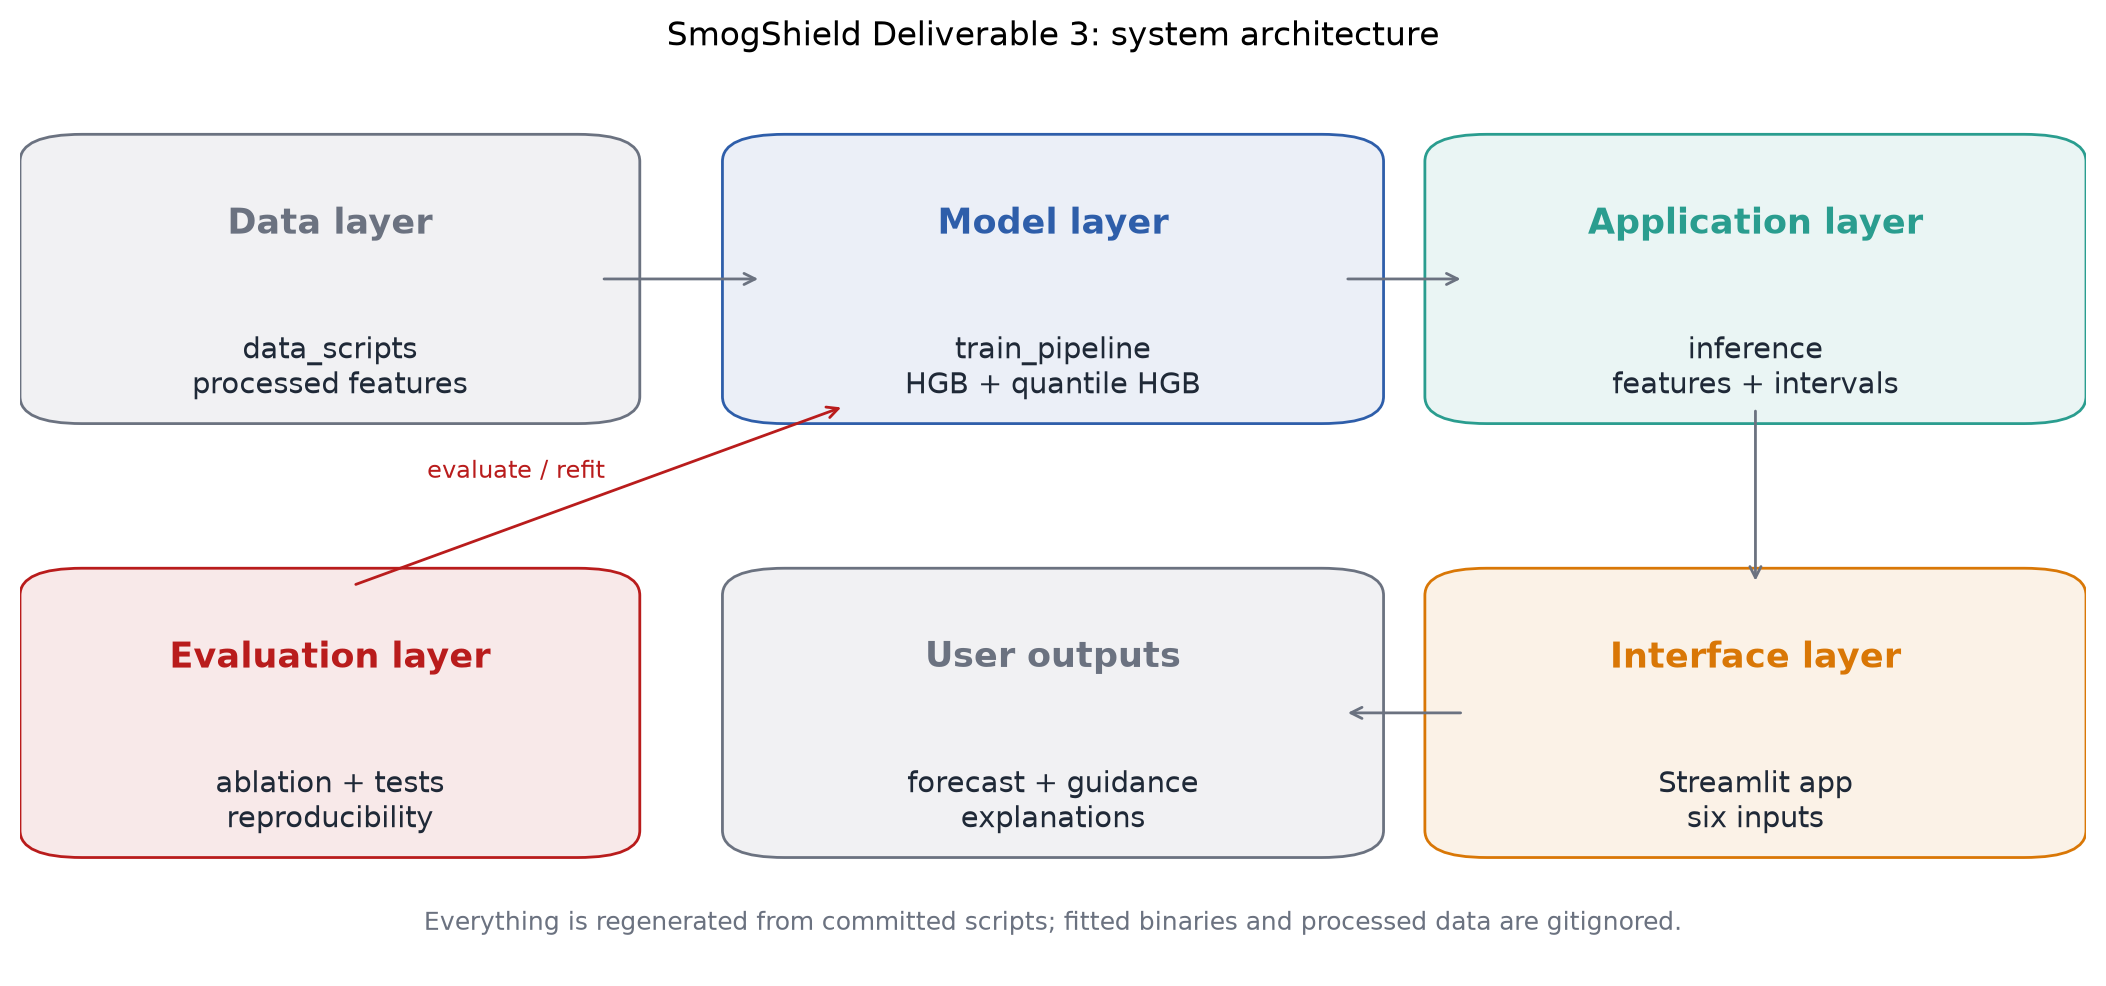
\includegraphics[width=\linewidth]{fig_architecture.png}
  \caption{Deliverable 3 system architecture. Fitted artifacts and processed
  data are regenerated from committed scripts; they are not committed to Git.}
  \label{fig:d3-architecture}
\end{figure}

Table~\ref{tab:artifacts} lists the runtime artifacts. The important policy is
that no fitted model binary and no processed data file is committed. The
repository contains the scripts that recreate them from fixed seeds. This is the
same policy used in Deliverable 2, extended to the four new pipelines and the
metadata file.

\begin{table}[htbp]
\centering
\footnotesize
\begin{tabular}{@{}L{5.4cm}L{3.5cm}L{3.5cm}L{2.6cm}@{}}
\toprule
\textbf{Artifact} & \textbf{Produced by} & \textbf{Consumed by} & \textbf{Committed?} \\
\midrule
\path{models/regression_pipeline.joblib} &
\texttt{src/train\_pipeline.py} & \texttt{src/inference.py} & No \\
\path{models/regression_q10_pipeline.joblib} &
\texttt{src/train\_pipeline.py} & \texttt{src/inference.py} & No \\
\path{models/regression_q90_pipeline.joblib} &
\texttt{src/train\_pipeline.py} & \texttt{src/inference.py} & No \\
\path{models/classification_pipeline.joblib} &
\texttt{src/train\_pipeline.py} & \texttt{src/inference.py} & No \\
\texttt{models/metadata.json} &
\texttt{src/train\_pipeline.py} & \texttt{src/inference.py}, app & No \\
\texttt{models/ablation.json} &
\texttt{src/ablation.py} & report, review & No \\
\path{data/processed/features_daily.csv} &
\path{data_scripts/09_build_features.py} &
\texttt{src/train\_pipeline.py} & No \\
\path{data/processed/pm25_hourly.csv} &
\path{data_scripts/02_clean_pm25_simple.py} &
\texttt{src/hourly.py} & No \\
\bottomrule
\end{tabular}
\caption{Runtime artifacts and their Git policy. The model directory has its own
\texttt{.gitignore}; the processed data directory is ignored at the repository
root.}
\label{tab:artifacts}
\end{table}

The architecture separates \emph{training} from \emph{serving}. The Streamlit
app imports \texttt{src.inference}, not the training modules. The inference
module loads the pipelines once, caches them in memory, and exposes a single
\texttt{predict()} call. If the artifacts are missing, it raises an error that
points the user at \texttt{python -m src.train\_pipeline}. This makes the failure
mode explicit rather than silently serving a stale or partial model.

\subsection{From six inputs to 46 features}
\label{sec:d3-features}

The model contract contains 46 raw features, which become 80 encoded columns
after one-hot encoding and missing-value indicators. The app collects only six
user-facing inputs. Table~\ref{tab:app-inputs} shows how each input is mapped
onto the model's real feature names.

\begin{table}[htbp]
\centering
\footnotesize
\begin{tabular}{@{}L{2.3cm}L{2.1cm}L{5.6cm}L{5.2cm}@{}}
\toprule
\textbf{App input} & \textbf{Unit} & \textbf{Derived model features} & \textbf{Default} \\
\midrule
Feature date & date &
\texttt{month}, \texttt{day\_of\_year}, \texttt{weekday},
\texttt{is\_weekend}, sin/cos terms, season dummies &
Today's date \\
Today's PM$_{2.5}$ & $\mu$g/m$^3$ &
\texttt{pm25}, \texttt{pm25\_log}, numeric \texttt{aqi}, lags 1--3,
rolling 3/7, difference &
Monthly historical median \\
Today's AQI category & seven raw labels &
\texttt{aqi\_category} (one-hot encoded) &
Derived from the default PM$_{2.5}$ \\
Temperature & $^\circ$C &
\texttt{temp\_mean\_c}, \texttt{temp\_max\_c}, \texttt{temp\_min\_c},
\texttt{temp\_mean\_c\_lag1} & 22 \\
Relative humidity & \% &
\texttt{humidity\_mean\_pct}, \texttt{humidity\_mean\_pct\_lag1} & 60 \\
Wind speed & km/h &
\texttt{wind\_speed\_mean\_kmh}, \texttt{wind\_speed\_max\_kmh},
\texttt{wind\_speed\_mean\_kmh\_lag1} & 7 \\
\bottomrule
\end{tabular}
\caption{The six user inputs and the model features they populate. Unlisted
features use training-set medians or modes.}
\label{tab:app-inputs}
\end{table}

The feature contract is filled in four steps. First, \texttt{build\_feature\_row}
starts from the training medians for numeric features and the training modes for
categorical features, both stored in \texttt{metadata.json}. Second, it maps the
six friendly inputs onto the model columns. Third, it derives the PM$_{2.5}$
history as a steady state: lags 1--3, the 3-day and 7-day rolling means, and the
day-to-day difference are set from today's PM$_{2.5}$, with the difference set to
zero. Fourth, explicit feature-column overrides are applied last. The
date-derived calendar features are computed from the selected feature date, not
from the forecast date; the forecast is always for the following day.

\paragraph{The numeric AQI fix.} The app does not ask for a numeric AQI. In an
early version the \texttt{aqi} feature therefore stayed at the training median of
165 even when the user entered a clean or hazardous PM$_{2.5}$ value. That was
internally inconsistent: the model saw a category and a PM$_{2.5}$ value that did
not correspond to the same AQI. The inference layer now derives \texttt{aqi} from
the entered PM$_{2.5}$ through the same US-EPA breakpoints used to build the
training labels. This is an inference-layer fix; the fitted pipelines and all
reported metrics are unchanged.

\paragraph{The category input is nearly inert.} The raw AQI category is a
categorical feature, but the numeric AQI and PM$_{2.5}$ carry almost all of the
signal. In an audit of the default November example, changing the category input
across all seven raw labels left the regression prediction identical to two
decimals (189.74 $\mu$g/m$^3$). The classifier's top probability moved only
between 0.9865 and 0.9910, and its arg-max stayed \emph{Very Unhealthy}. This is
not a bug in the UI; it is a property of the fitted model. The app keeps the
category input because it is part of the model contract and because the raw
seven-label vocabulary is familiar to users, but the report does not claim that
the category selector drives the forecast.

\begin{table}[htbp]
\centering
\small
\begin{tabular}{@{}lrr@{}}
\toprule
\textbf{Input category} & \textbf{Regression PM$_{2.5}$} &
\textbf{Classifier top label (probability)} \\
\midrule
Good & 189.74 & Very Unhealthy (0.991) \\
Moderate & 189.74 & Very Unhealthy (0.991) \\
Unhealthy for Sensitive & 189.74 & Very Unhealthy (0.991) \\
Unhealthy & 189.74 & Very Unhealthy (0.987) \\
Very Unhealthy & 189.74 & Very Unhealthy (0.991) \\
Hazardous (301--400) & 189.74 & Very Unhealthy (0.991) \\
Hazardous (401--500) & 189.74 & Very Unhealthy (0.991) \\
\bottomrule
\end{tabular}
\caption{Category-input audit for the default November example (PM$_{2.5}$ =
234.2, temperature 22$^\circ$C, humidity 60\%, wind 7 km/h, 12 November 2026).
The numeric PM$_{2.5}$ and derived AQI dominate; the category selector is nearly
inert.}
\label{tab:category-audit}
\end{table}

\paragraph{Feature groups.} Table~\ref{tab:feature-groups} groups the 46 raw
features. The 12 history features are the inputs that the ablation calls
``history only.'' Adding 17 calendar features gives the 29-feature set; adding
17 weather features gives the full 46-feature set. This is the same nested
design used in the Deliverable 3 ablation.

\begin{table}[htbp]
\centering
\small
\begin{tabular}{@{}L{3.4cm}rL{9.2cm}@{}}
\toprule
\textbf{Feature group} & \textbf{Raw count} & \textbf{Examples} \\
\midrule
Air quality and history & 12 &
\texttt{pm25}, \texttt{aqi}, \texttt{aqi\_category}, \texttt{pm25\_log},
lags 1--3, rolling 3/7, difference, data-quality flags \\
Calendar and events & 17 &
month, day-of-year, weekday, weekend, sin/cos terms, season dummies,
Ramadan, Eid, public holiday \\
Weather & 17 &
temperature (mean/max/min/lag), humidity (mean/lag), dew point, pressure
(mean/lag), wind (mean/max/lag/direction), rain, solar radiation, cloud cover \\
\midrule
Total & 46 & 80 encoded columns after preprocessing \\
\bottomrule
\end{tabular}
\caption{The nested feature groups. The ablation uses the 12-, 29-, and
46-feature sets with the same frozen hyperparameters.}
\label{tab:feature-groups}
\end{table}

\subsection{The forecast screen}
\label{sec:d3-ui}

Figure~\ref{fig:d3-ui} shows the flow of the forecast screen. The user enters
the six values in a two-column form. Pressing \emph{Forecast next day} calls
\texttt{inference.predict()} and returns three rows of output. The first row
shows the predicted PM$_{2.5}$, the AQI implied by that PM$_{2.5}$, and the
implied AQI category. The second row shows the classifier's category, its
confidence, and the persistence value. The third block shows the 80\% interval,
the guidance banner, the local sensitivity chart, and the expanders for global
importance, winter stagnation, and the hourly profile.

\begin{figure}[htbp]
  \centering
  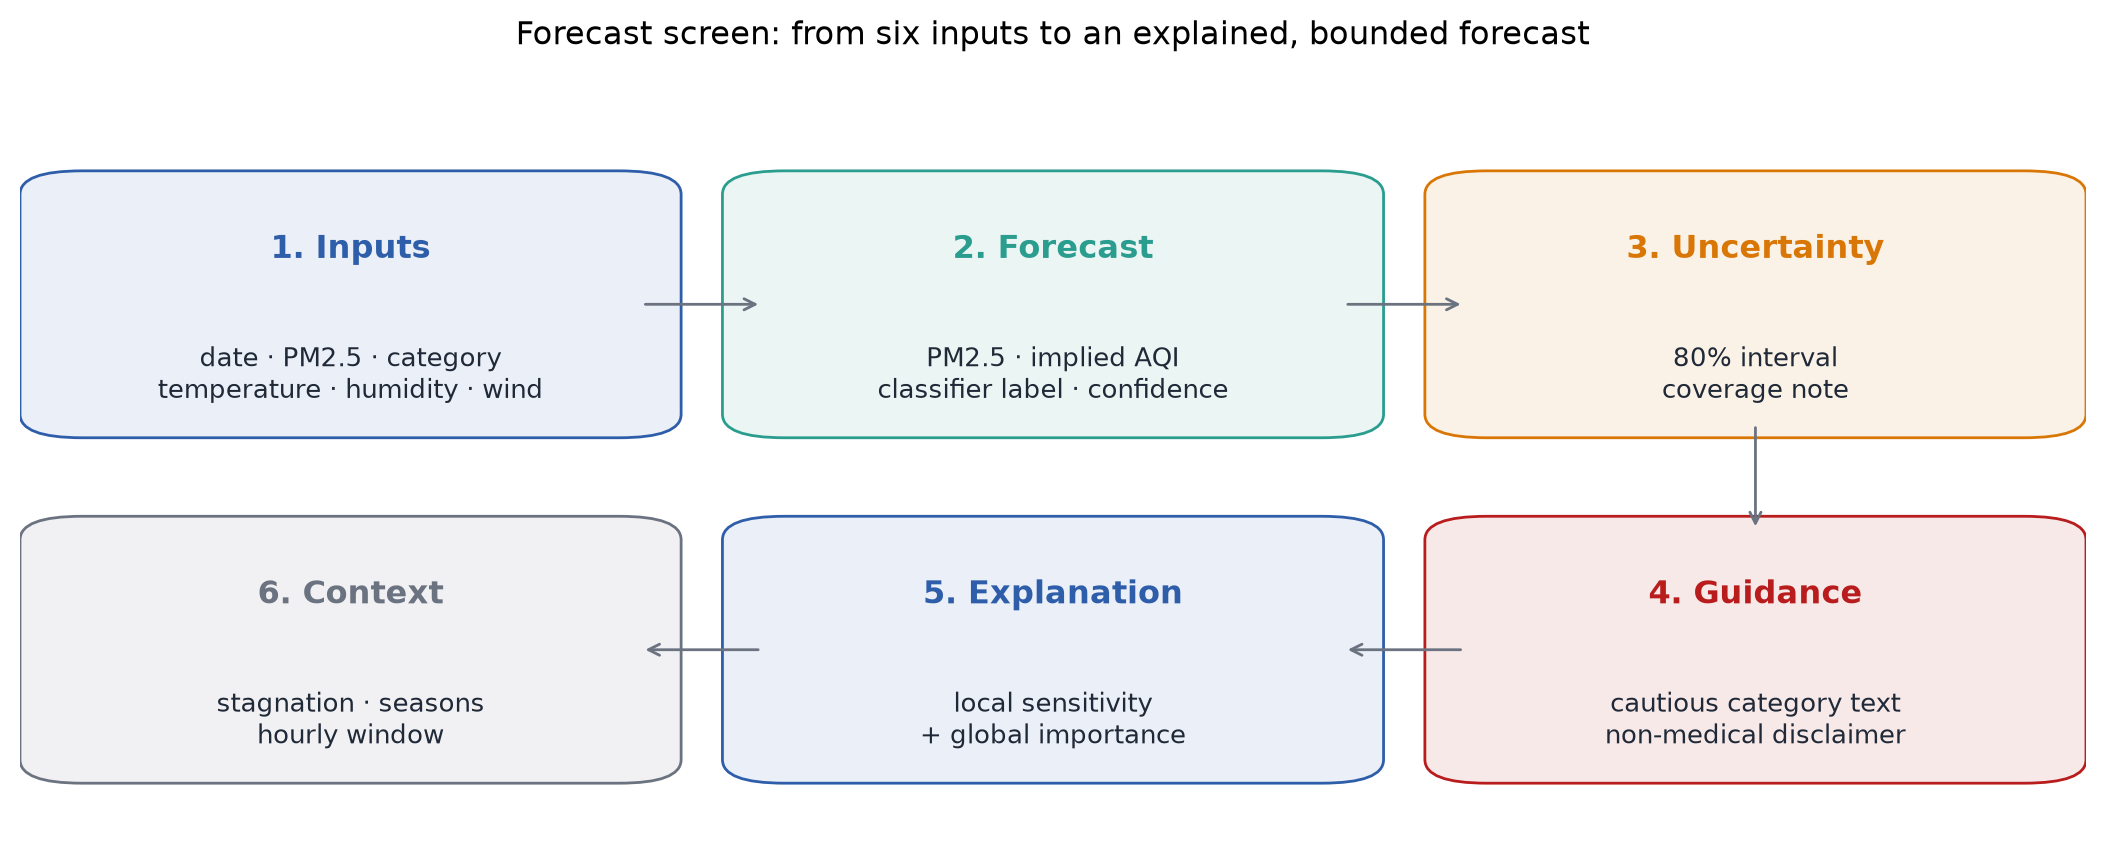
\includegraphics[width=\linewidth]{fig_ui_flow.png}
  \caption{The forecast screen in six steps. The interface is a single
  Streamlit page; the expanders keep the historical context available without
  crowding the primary forecast.}
  \label{fig:d3-ui}
\end{figure}

Table~\ref{tab:ui-outputs} explains each output. The table is intentionally
redundant with the app: a user should not have to infer what a card means, and a
reviewer should be able to check that the screen is not hiding a weaker result.

\begin{table}[htbp]
\centering
\footnotesize
\begin{tabular}{@{}L{3.1cm}L{6.1cm}L{5.9cm}@{}}
\toprule
\textbf{Output} & \textbf{What it shows} & \textbf{How to read it} \\
\midrule
Predicted PM$_{2.5}$ & Regression point forecast for tomorrow &
A single number in $\mu$g/m$^3$; not a guarantee \\
AQI implied by PM$_{2.5}$ & US-EPA AQI computed from the predicted PM$_{2.5}$ &
Monotonic in the prediction; uses the same breakpoints as the labels \\
Implied category & EPA category of the implied AQI &
The more defensible category view because the classifier was weaker than
persistence \\
Classifier category and confidence & Six-class HGB arg-max and its probability &
A separate model; biased toward \emph{Unhealthy} \\
Persistence & Tomorrow = today, for PM$_{2.5}$ and category &
The baseline the model must beat; shown on every forecast \\
80\% interval & Calibrated central interval for next-day PM$_{2.5}$ &
A range, not a worst case; test coverage is 77.0\% \\
Local sensitivity & Change in the forecast when one input is increased &
A finite difference, not a causal effect \\
Global importance & Permutation importance on validation &
Which features the model relies on overall \\
Winter stagnation & Share of stagnant winter days and their mean PM$_{2.5}$ &
Descriptive history, not a today-specific forecast \\
Best time outdoors & Hour-of-day and seasonal PM$_{2.5}$ profile &
Station-specific history; winter afternoons remain polluted \\
Guidance & Cautious, non-medical advice for the implied category &
Follow official advisories; not medical advice \\
Disagreement warning & Appears when the two category views differ &
Explains which view the app recommends and why \\
\bottomrule
\end{tabular}
\caption{The forecast screen outputs and their interpretation.}
\label{tab:ui-outputs}
\end{table}

The interface was exercised with Streamlit's application test harness. The
AppTest run reported no exceptions, four charts, and three expanders. This is a
smoke test, not a usability study: it confirms that the page renders and the
main branches execute, not that the wording is clear to a first-time user.

\subsection{Prediction intervals}
\label{sec:d3-intervals}

A point forecast is not enough for a decision. The app therefore trains two
additional HGB models with quantile loss, one at the 10th percentile and one at
the 90th percentile, and combines them into an 80\% central prediction interval.
The bounds are forced to contain the point forecast and are then widened by a
calibration factor chosen on the validation split. On this dataset the factor is
1.00, so no widening was needed. Validation coverage is 80.3\%; test coverage is
77.0\%. The test split is used only to report coverage, never to choose the
factor.

\begin{table}[htbp]
\centering
\small
\begin{tabular}{@{}lr@{}}
\toprule
\textbf{Property} & \textbf{Value} \\
\midrule
Nominal level & 80\% \\
Quantiles & 10th and 90th \\
Calibration scale & 1.00 \\
Validation coverage & 80.3\% \\
Test coverage & 77.0\% \\
Tuning rule & Validation only; test reported, never tuned \\
\bottomrule
\end{tabular}
\caption{The 80\% prediction interval. The test coverage is below nominal, which
is reported rather than hidden.}
\label{tab:interval}
\end{table}

Figure~\ref{fig:d3-interval} shows the nominal-versus-empirical coverage and the
default November example. The default is deliberately a polluted day: today's
PM$_{2.5}$ is the historical November median, 234.2 $\mu$g/m$^3$; the app
forecasts 189.74 $\mu$g/m$^3$ with an interval of 133.8--294.1 $\mu$g/m$^3$.
The interval spans categories from \emph{Unhealthy} to \emph{Hazardous
(301--400)}, even though the point forecast is \emph{Very Unhealthy}. That width
is the honest message: the model is not precise enough to support a single
category claim.

\begin{figure}[htbp]
  \centering
  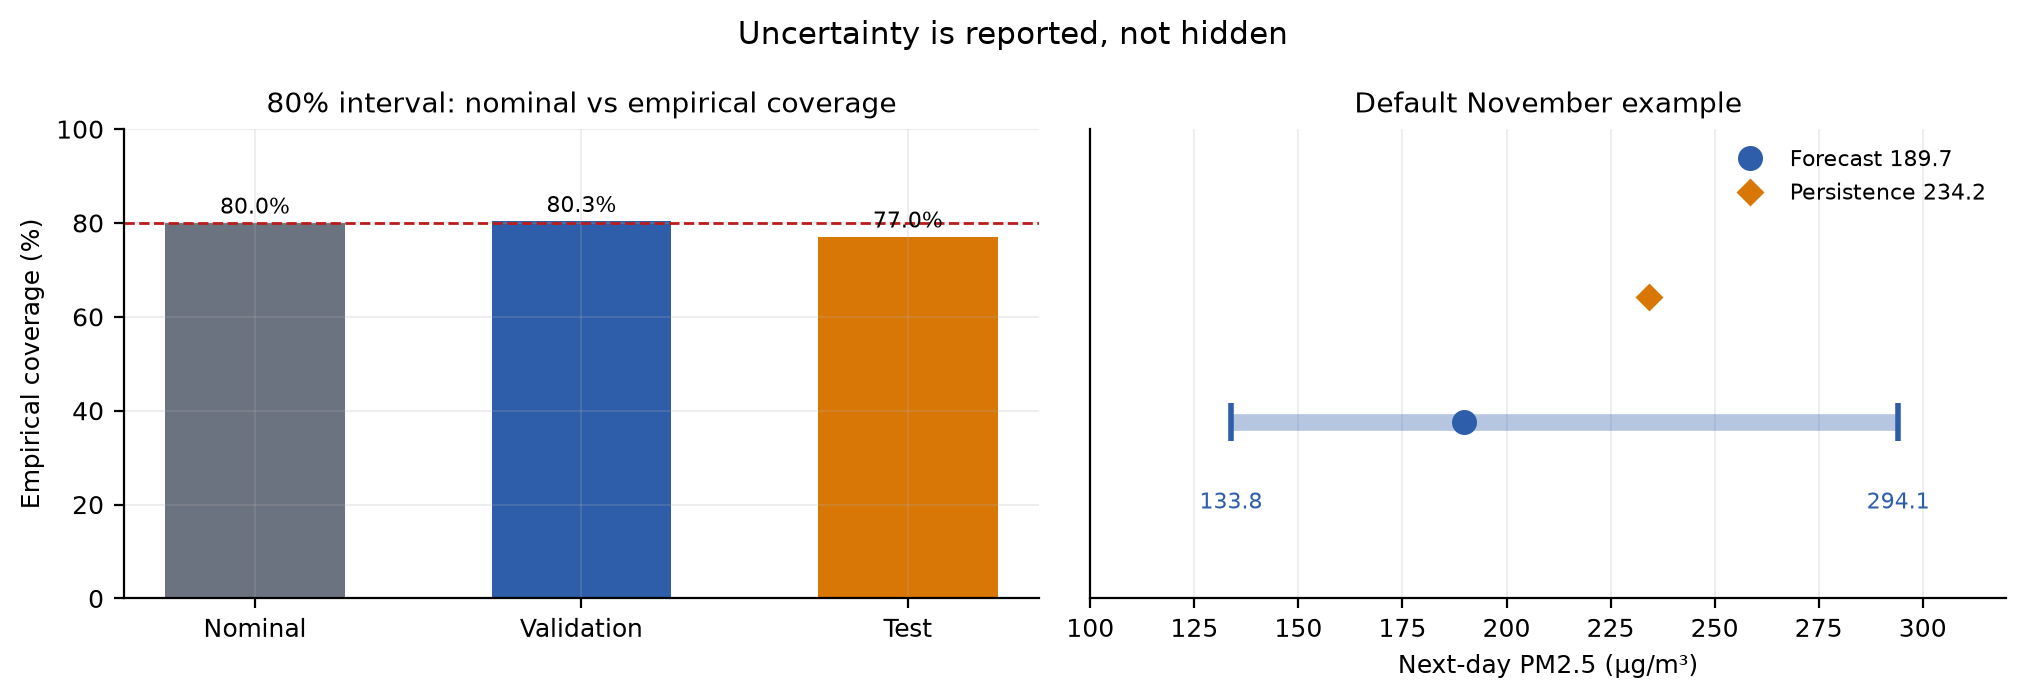
\includegraphics[width=\linewidth]{fig_interval.png}
  \caption{Left: nominal 80\% coverage versus validation and test coverage.
  Right: the default November forecast and its 80\% interval, compared with
  persistence. The interval is wide because the model is uncertain, not because
  the app is hiding a point estimate.}
  \label{fig:d3-interval}
\end{figure}

The interval is a central interval for the \emph{next-day PM$_{2.5}$ observation},
not a confidence interval for the model's mean prediction. It does not include
model-selection uncertainty, distribution shift, or the error introduced by the
steady-state feature assumption. A future version should add conformal
prediction and a separate interval for the AQI category.

\subsection{Explanations: global and local}
\label{sec:d3-explanations}

The app provides two explanations with different scopes. The global explanation
uses permutation importance on the validation split: one feature at a time is
shuffled, and the increase in RMSE (regression) or the drop in macro-F1
(classification) is recorded. The local explanation perturbs one input for the
current forecast and reports the change in the predicted PM$_{2.5}$.

\paragraph{Global view.} Figure~\ref{fig:d3-importance} and
Table~\ref{tab:importance} show the top features. For regression, today's
PM$_{2.5}$ is dominant (increase in RMSE 14.51), followed by the numeric AQI
(4.20), day-of-year (4.15), lag-1 PM$_{2.5}$ (2.93), and wind direction (2.50).
For classification, the top features are PM$_{2.5}$ (drop in macro-F1 0.0786),
wind direction (0.0672), pressure (0.0506), numeric AQI (0.0495), and the
day-of-year cosine (0.0407). The presence of day-of-year and seasonal terms is
consistent with the strong winter cycle.

The ranking is descriptive, not causal. Permutation importance breaks the
relationship between a feature and its correlated neighbours. Shuffling
\texttt{pm25} while leaving the lags intact can overstate its unique
contribution; conversely, a feature that is redundant with another may look
unimportant. The report uses the ranking to explain what the model relies on,
not to claim that changing a feature would change the outcome by that amount.

\begin{figure}[htbp]
  \centering
  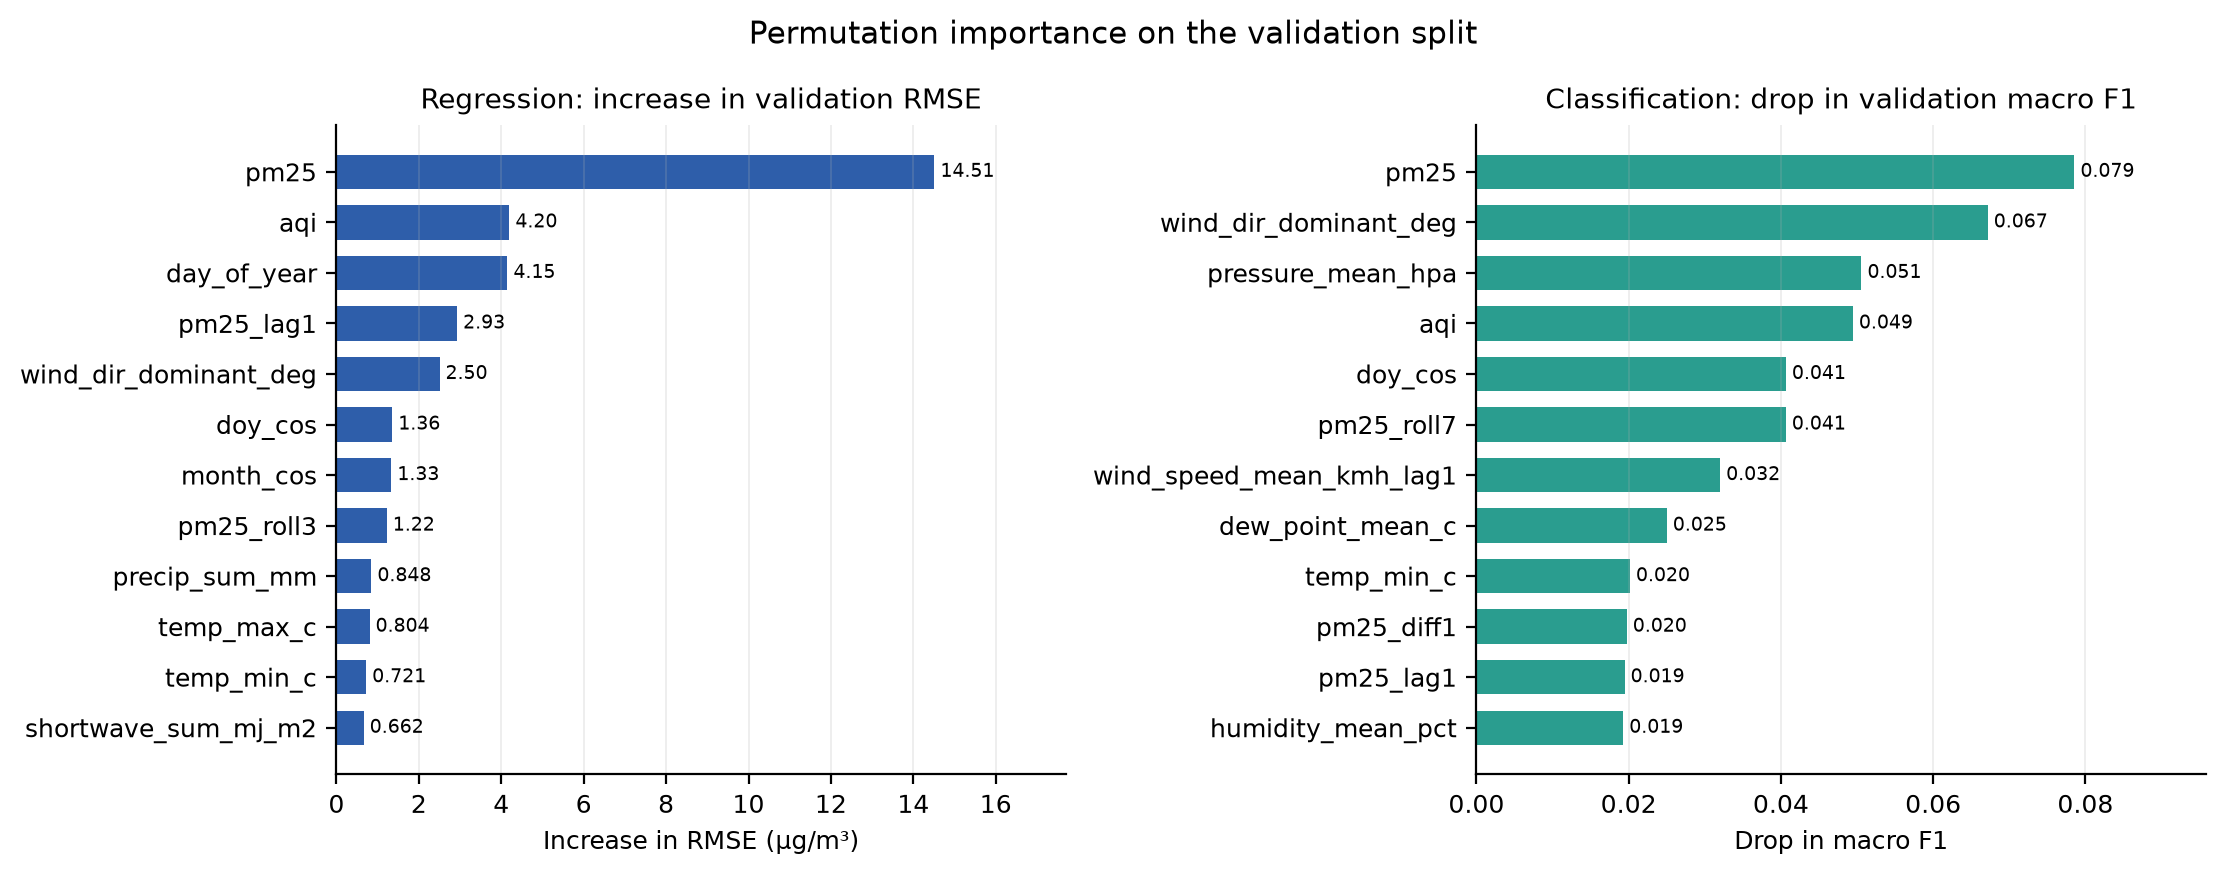
\includegraphics[width=\linewidth]{fig_importance.png}
  \caption{Permutation importance on the validation split. Regression scores are
  the increase in RMSE when a feature is shuffled; classification scores are the
  drop in macro-F1. Correlated features share credit, so the ranking is not a
  causal decomposition.}
  \label{fig:d3-importance}
\end{figure}

\begin{table}[htbp]
\centering
\footnotesize
\begin{tabular}{@{}rlrrl r@{}}
\toprule
\multicolumn{3}{c}{\textbf{Regression (increase in RMSE)}} &
\multicolumn{3}{c}{\textbf{Classification (drop in macro-F1)}} \\
\cmidrule(lr){1-3}\cmidrule(lr){4-6}
\textbf{Rank} & \textbf{Feature} & \textbf{Value} &
\textbf{Rank} & \textbf{Feature} & \textbf{Value} \\
\midrule
1 & \texttt{pm25} & 14.51 & 1 & \texttt{pm25} & 0.0786 \\
2 & \texttt{aqi} & 4.20 & 2 & \texttt{wind\_dir\_dominant\_deg} & 0.0672 \\
3 & \texttt{day\_of\_year} & 4.15 & 3 & \texttt{pressure\_mean\_hpa} & 0.0506 \\
4 & \texttt{pm25\_lag1} & 2.93 & 4 & \texttt{aqi} & 0.0495 \\
5 & \texttt{wind\_dir\_dominant\_deg} & 2.50 & 5 & \texttt{doy\_cos} & 0.0407 \\
6 & \texttt{doy\_cos} & 1.36 & 6 & \texttt{pm25\_roll7} & 0.0406 \\
7 & \texttt{month\_cos} & 1.33 & 7 & \texttt{wind\_speed\_mean\_kmh\_lag1} & 0.0320 \\
8 & \texttt{pm25\_roll3} & 1.22 & 8 & \texttt{dew\_point\_mean\_c} & 0.0250 \\
\bottomrule
\end{tabular}
\caption{Top eight permutation-importance features for the two tasks.}
\label{tab:importance}
\end{table}

\paragraph{Local view.} The local explanation answers a narrower question: for
\emph{this} forecast, what happens if one input is increased by a fixed amount?
The app perturbs four inputs: PM$_{2.5}$ by +25 $\mu$g/m$^3$, temperature by
+5$^\circ$C, humidity by +10 percentage points, and wind speed by +5 km/h. The
PM$_{2.5}$ step is larger than the others because HGB predictions are piecewise
constant: a +10 step often stays inside the same leaf and reports a misleading
0.0. A +25 step crosses splits more reliably, but it is still a finite
difference, not a smooth slope.

Table~\ref{tab:local} shows the local explanation for the default November
example. A +25 $\mu$g/m$^3$ increase in today's PM$_{2.5}$ raises the forecast by
38.68 $\mu$g/m$^3$; a +5$^\circ$C temperature increase raises it by 18.41; a
+5 km/h wind increase lowers it by 7.08; and a +10-point humidity increase
lowers it by 0.43. The wind sign matches the physical intuition that stronger
wind disperses pollution. The temperature sign is local and counter-intuitive
at first glance; it should not be read as a causal effect, because temperature
is correlated with season, pressure, and the winter inversion regime.

\begin{table}[htbp]
\centering
\small
\begin{tabular}{@{}lrr@{}}
\toprule
\textbf{Input change} & \textbf{Change in forecast} & \textbf{Direction} \\
\midrule
PM$_{2.5}$ +25 $\mu$g/m$^3$ & +38.68 & Higher forecast \\
Temperature +5$^\circ$C & +18.41 & Higher forecast \\
Wind +5 km/h & $-7.08$ & Lower forecast \\
Humidity +10 points & $-0.43$ & Slightly lower forecast \\
\bottomrule
\end{tabular}
\caption{Local sensitivity for the default November example (point forecast
189.74 $\mu$g/m$^3$). The values are one-at-a-time finite differences, not
causal effects.}
\label{tab:local}
\end{table}

The app ranks the four bars by absolute effect. A zero-length bar is possible
even for an important feature if the perturbation stays inside a leaf; the
larger PM$_{2.5}$ step reduces, but does not eliminate, that artifact. A
Shapley-value decomposition would be a more principled local explanation and is
left as future work.

\subsection{Seasonal defaults and historical context}
\label{sec:d3-seasonal}

The app opens on a seasonally plausible scenario rather than a fixed clean-day
value. The initial PM$_{2.5}$ is the historical median for the current calendar
month, and the initial category is derived from that PM$_{2.5}$ through the EPA
breakpoints. On 12 November 2026 the default is 234.2 $\mu$g/m$^3$ and
\emph{Very Unhealthy}; the forecast is 189.74 $\mu$g/m$^3$, still
\emph{Very Unhealthy}, with a persistence value of 234.2 $\mu$g/m$^3$.

This choice matters for the demo. A fixed 60 $\mu$g/m$^3$ default would open the
app on a moderately polluted day that is not representative of November in
Lahore. The monthly medians in Table~\ref{tab:monthly} and
Figure~\ref{fig:d3-seasonal} show the size of the seasonal swing: the median is
253.3 $\mu$g/m$^3$ in December, 234.2 in November, and 44.4 in August. The
default is a starting point, not a live reading; the user can override it.

\begin{table}[htbp]
\centering
\small
\begin{tabular}{@{}lrlr@{}}
\toprule
\textbf{Month} & \textbf{Median PM$_{2.5}$} &
\textbf{Month} & \textbf{Median PM$_{2.5}$} \\
\midrule
January & 216.5 & July & 47.5 \\
February & 145.0 & August & 44.4 \\
March & 83.7 & September & 62.1 \\
April & 59.8 & October & 119.1 \\
May & 70.9 & November & 234.2 \\
June & 67.0 & December & 253.3 \\
\bottomrule
\end{tabular}
\caption{Historical monthly median PM$_{2.5}$ ($\mu$g/m$^3$), computed from
physically valid daily values. The app uses the current month's median as its
initial PM$_{2.5}$ default.}
\label{tab:monthly}
\end{table}

\begin{figure}[htbp]
  \centering
  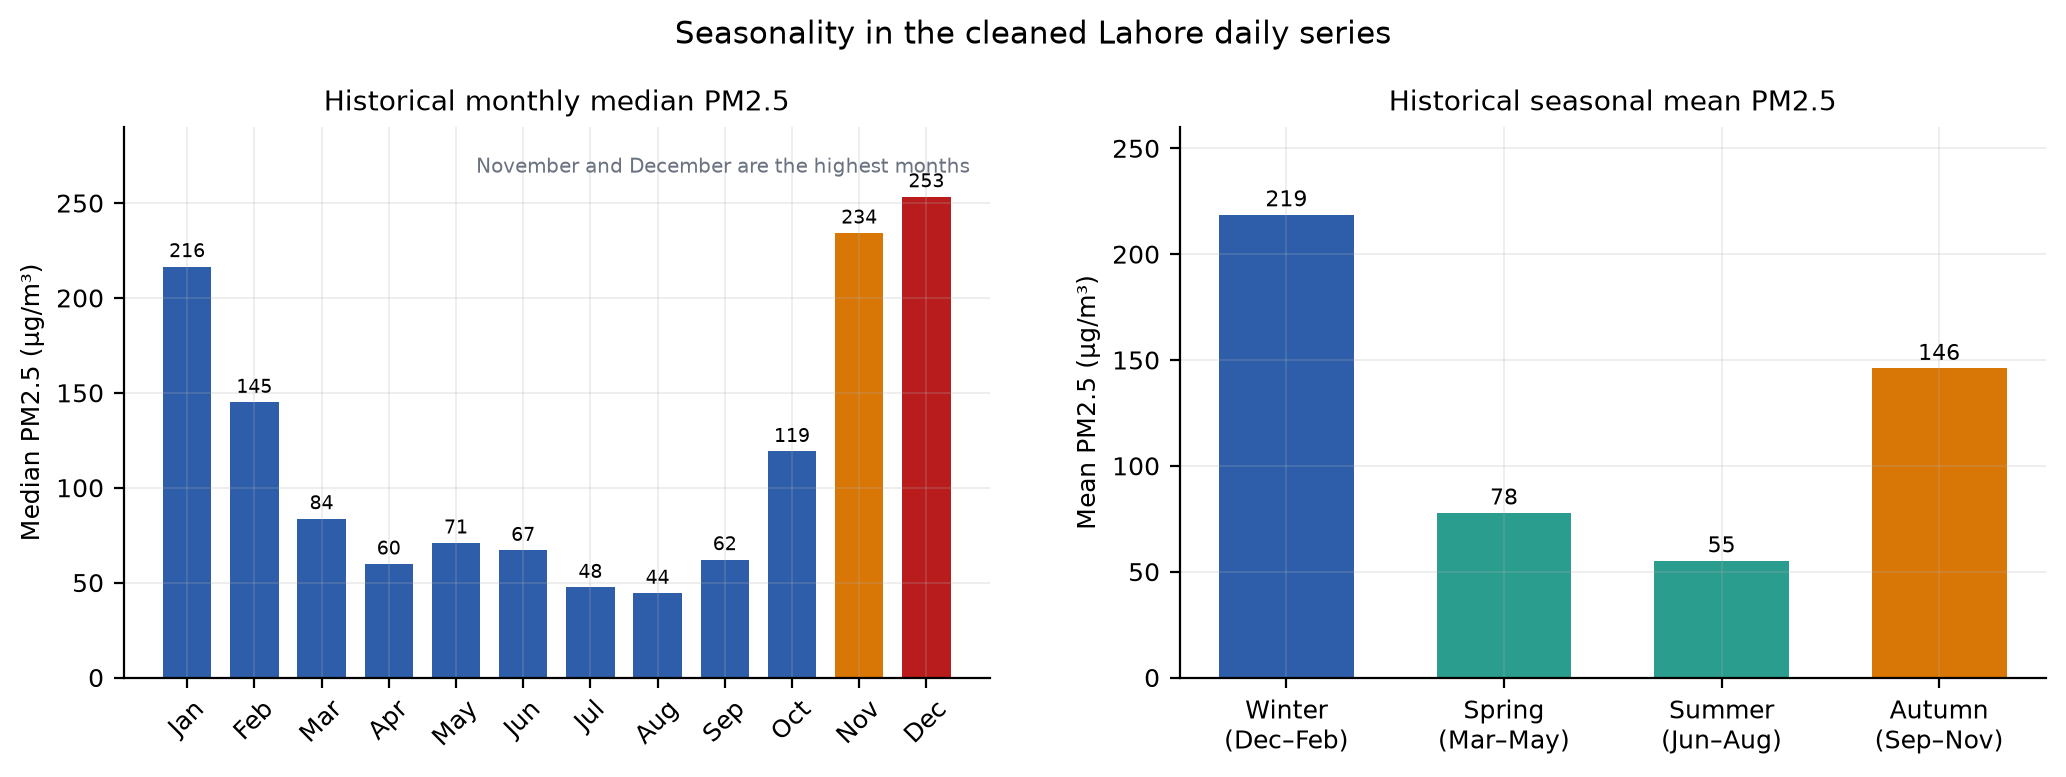
\includegraphics[width=\linewidth]{fig_seasonal.png}
  \caption{Historical monthly medians and seasonal means. November and December
  are the highest months; summer is much cleaner. These are descriptive
  statistics from one station, not a forecast.}
  \label{fig:d3-seasonal}
\end{figure}

\paragraph{Winter stagnation.} The app also reports a simple historical pattern.
A winter day (December--February) is labelled \emph{stagnant} when its mean wind
speed is in the winter lower quartile and it recorded at most 0.5 mm of rain. Of
407 winter days, 100 (24.6\%) meet the definition. Their mean PM$_{2.5}$ is
294.9 $\mu$g/m$^3$, versus 193.7 $\mu$g/m$^3$ on better-ventilated days, a
difference of +52.2\%. The winter wind quartile threshold is 5.2 km/h. This is a
descriptive proxy for stagnation, not a dispersion model, and it should not be
read as a causal estimate of the effect of wind.

\begin{table}[htbp]
\centering
\small
\begin{tabular}{@{}lr@{}}
\toprule
\textbf{Quantity} & \textbf{Value} \\
\midrule
Winter days (Dec--Feb) & 407 \\
Stagnant days & 100 (24.6\%) \\
Winter wind lower quartile & 5.2 km/h \\
Mean PM$_{2.5}$ on stagnant days & 294.9 $\mu$g/m$^3$ \\
Mean PM$_{2.5}$ on ventilated days & 193.7 $\mu$g/m$^3$ \\
Difference & +52.2\% \\
\bottomrule
\end{tabular}
\caption{Winter stagnation summary. The definition is descriptive and the
difference is associational.}
\label{tab:stagnation}
\end{table}

\paragraph{Seasonal means.} The seasonal means are 218.6 $\mu$g/m$^3$ in winter,
146.0 in autumn, 77.7 in spring, and 55.1 in summer. These values are the
context for the app's guidance: a November forecast that looks lower than today
can still be \emph{Very Unhealthy}, and a winter afternoon that is cleaner than
the morning can still be far above the WHO guideline. The app says this
explicitly rather than implying that timing solves the problem.

\subsection{The hourly profile}
\label{sec:d3-hourly}

The hourly card uses 36,820 valid hourly observations from the Lahore US
Diplomatic Post sensor, covering 2019-05-23 to 2025-02-18. The overall cleanest
three-hour window is 14:00--16:59, with a mean PM$_{2.5}$ of 85.2
$\mu$g/m$^3$; the worst hour is 22:00, with 138.4 $\mu$g/m$^3$. The afternoon
minimum holds in every season, but the winter version of the same window still
averages 155.4 $\mu$g/m$^3$, versus 41.2 in spring, 44.4 in summer, and 90.8 in
autumn. Timing helps; it does not make winter air safe.

\begin{table}[htbp]
\centering
\small
\begin{tabular}{@{}lr@{}}
\toprule
\textbf{Window or season} & \textbf{Mean PM$_{2.5}$} \\
\midrule
Cleanest overall window (14:00--16:59) & 85.2 $\mu$g/m$^3$ \\
Worst hour (22:00) & 138.4 $\mu$g/m$^3$ \\
Winter cleanest window (14:00--16:59) & 155.4 $\mu$g/m$^3$ \\
Spring cleanest window & 41.2 $\mu$g/m$^3$ \\
Summer cleanest window & 44.4 $\mu$g/m$^3$ \\
Autumn cleanest window & 90.8 $\mu$g/m$^3$ \\
\bottomrule
\end{tabular}
\caption{The hourly profile. The source is a single station and the values are
descriptive history, not a today-specific hourly forecast.}
\label{tab:hourly}
\end{table}

\begin{figure}[htbp]
  \centering
  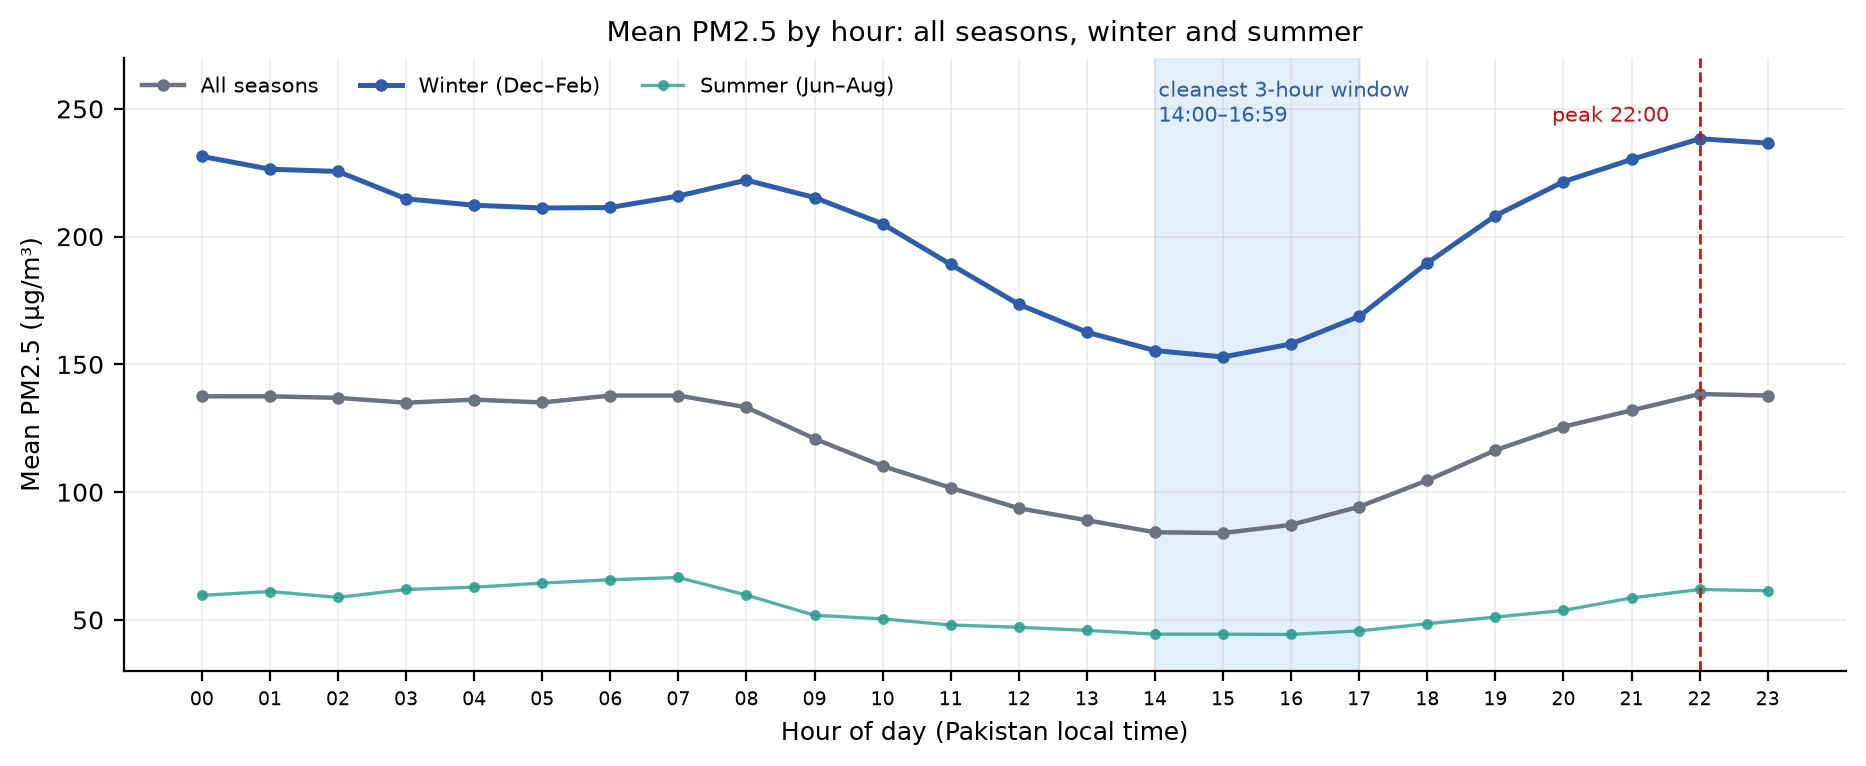
\includegraphics[width=\linewidth]{fig_hourly.png}
  \caption{Mean PM$_{2.5}$ by hour for all seasons, winter, and summer. The
  shaded window is the overall cleanest three hours; the dashed line marks the
  worst hour. Winter afternoons remain polluted.}
  \label{fig:d3-hourly}
\end{figure}

The card carries a caveat in the app: it is a descriptive station history in
Pakistan local time, not a today-specific forecast. The hourly source file is not
committed; if it is absent, the app omits the card and the rest of the pipeline
still runs.

\subsection{Persistence, guidance, and the honesty contract}
\label{sec:d3-honesty}

The app displays persistence on every forecast. Table~\ref{tab:persistence}
repeats the comparison that drives the report's framing. On the test split, the
regression's RMSE is 64.92 versus 64.82 for persistence, a difference of 0.10
$\mu$g/m$^3$ and a skill score of $-0.0016$. The classifier's macro-F1 is 0.4780
versus 0.5157 for persistence, even though the classifier's accuracy is slightly
higher (0.5856 versus 0.5676). The accuracy/macro-F1 split is the key: accuracy
is dominated by the common \emph{Unhealthy} class, while macro-F1 gives the rare
hazardous classes equal weight.

\begin{table}[htbp]
\centering
\small
\begin{tabular}{@{}lrrrr@{}}
\toprule
\textbf{Task and model} & \textbf{Validation} & \textbf{Test} &
\textbf{Persistence validation} & \textbf{Persistence test} \\
\midrule
Regression, HGB RMSE & 45.62 & 64.92 & 51.55 & 64.82 \\
Classification, HGB macro-F1 & 0.4941 & 0.4780 & 0.4766 & 0.5157 \\
\bottomrule
\end{tabular}
\caption{The frozen model versus persistence. The regression ties persistence on
test; the classifier loses on macro-F1. Ridge reached a lower test RMSE (62.10)
but was not the validation-selected model, so it is not used.}
\label{tab:persistence}
\end{table}

When the two category views disagree, the app shows a warning and says that the
implied category is the more defensible view because the classifier was weaker
than persistence on test. This is a deliberate design choice: hiding the
disagreement would make the interface look more confident than the evidence
supports.

\paragraph{Guidance.} The guidance text is keyed to the regression-implied
category and is cautious and non-medical. Table~\ref{tab:guidance} lists the
headlines. Every message carries a disclaimer that it is not a substitute for
official health advice. The app does not tell a user that it is safe to exercise;
it tells a user when to consider reducing exertion and when to avoid prolonged
outdoor activity.

\begin{table}[htbp]
\centering
\small
\begin{tabular}{@{}L{5.2cm}L{9.0cm}@{}}
\toprule
\textbf{Implied category} & \textbf{Headline} \\
\midrule
Good/Moderate & Air quality is relatively favourable. \\
Unhealthy for Sensitive & Sensitive groups should take care. \\
Unhealthy & Consider reducing outdoor exertion. \\
Very Unhealthy & Avoid prolonged outdoor activity. \\
Hazardous (301--400) & Avoid outdoor activity. \\
Hazardous (401--500) & Avoid outdoor activity. \\
\bottomrule
\end{tabular}
\caption{Cautious guidance by implied AQI category. The app adds a non-medical
disclaimer to every message.}
\label{tab:guidance}
\end{table}

\subsection{Tests and reproducibility}
\label{sec:d3-tests}

The application layer has 14 unit tests. They cover the EPA breakpoints and
category mapping, the feature schema and defaults, the interval bounds, the
local explanation, the guidance dictionary, the seasonal/stagnation patterns,
the monthly medians, and the hourly profile. The Streamlit AppTest adds a render
smoke test: no exceptions, four charts, and three expanders.

\begin{table}[htbp]
\centering
\small
\begin{tabular}{@{}L{4.4cm}L{10.0cm}@{}}
\toprule
\textbf{Test area} & \textbf{What is checked} \\
\midrule
AQI conversion & Breakpoints and category labels match the training labels \\
Feature contract & The app builds the expected columns, with the expected defaults \\
Intervals & Bounds contain the point forecast and respect the calibration factor \\
Explanation & Sensitivity returns the four perturbations in the expected shape \\
Guidance & Every category has a headline, detail, and disclaimer \\
Patterns & Stagnation, seasonal means, monthly medians, and hourly profile are present \\
App render & AppTest reports no exceptions, four charts, and three expanders \\
\bottomrule
\end{tabular}
\caption{Test coverage for the Deliverable 3 application layer.}
\label{tab:tests}
\end{table}

The reproducibility check is stronger than the test suite. Refitting the D3
pipelines from the committed script reproduces the Deliverable 2 metrics exactly:
regression validation/test RMSE 45.6243/64.9198, persistence 51.5457/64.8175;
classification validation/test macro-F1 0.4941/0.4780, persistence
0.4766/0.5157; interval coverage 80.3\%/77.0\%. The D2 code and report were not
edited. The D3 training script adds the two classifier settings that were needed
to match D2 exactly: balanced class weights and disabled early stopping. The
model itself is unchanged.

\section{Phase 6: Final Evaluation and Discussion}
\label{sec:phase6}

This section integrates the six phases, evaluates the application as a whole,
and states what the project can and cannot claim. The central finding is
negative but useful: the frozen model does not beat persistence, and the
application is designed to say so.

\subsection{Integrated results across phases}
\label{sec:integrated}

Table~\ref{tab:integrated} summarizes the delivered phases. The project moved
from a problem definition and a documented dataset, through a validation-selected
model and a bias analysis, to an application and an honest final evaluation.
The model scores did not change between Deliverable 2 and Deliverable 3.

\begin{table}[htbp]
\centering
\footnotesize
\begin{tabular}{@{}L{2.2cm}L{4.7cm}L{7.5cm}@{}}
\toprule
\textbf{Phase} & \textbf{Main output} & \textbf{Headline} \\
\midrule
Phase 1 & Problem definition and objectives &
1,506 valid days; only 9 Good days (0.6\%); 73.2\% Unhealthy or worse \\
Phase 2 & Data foundations and EDA &
2,113 daily rows, 63 columns, 2019-05-23 to 2025-03-04; one station \\
Phase 3 & Model development and selection &
HGB selected on validation: RMSE 45.62, macro-F1 0.4941 \\
Phase 4 & Evaluation and bias analysis &
Test RMSE 64.92 vs persistence 64.82; macro-F1 0.478 vs 0.516; severe-tail
errors are the largest \\
Phase 5 & Application and explainability &
Six inputs, two category views, 80\% interval, local/global explanations,
seasonal defaults, stagnation, hourly profile \\
Phase 6 & Final evaluation and discussion &
Ablation, backtest, limitations, reproducibility, and an honest verdict: the
app demonstrates the pipeline; it does not beat persistence \\
\bottomrule
\end{tabular}
\caption{Integrated results across the six phases.}
\label{tab:integrated}
\end{table}

The contribution is not a new accuracy record. It is an end-to-end, reproducible
system that makes a difficult result visible: a strong one-day persistence
baseline is hard to beat with the available features, and the remaining errors
are concentrated on the most severe pollution days, which are exactly the days
that matter most for public health.

\subsection{Ablation: do weather and calendar features help?}
\label{sec:ablation}

The ablation refits both tasks on three nested feature sets with the frozen
hyperparameters: history only (12 features), history plus calendar (29), and the
full set (46). Test metrics are reported but never used to choose a set. The
results are in Table~\ref{tab:ablation} and Figure~\ref{fig:d3-ablation}.

\begin{table}[htbp]
\centering
\footnotesize
\setlength{\tabcolsep}{4.5pt}
\begin{tabular}{@{}lrrrrr@{}}
\toprule
\textbf{Feature set} & \textbf{Feat.} &
\textbf{Reg. val} & \textbf{Reg. test} &
\textbf{Clf. val} & \textbf{Clf. test} \\
\midrule
History only & 12 & 52.18 & 63.88 & 0.4663 & 0.4715 \\
History + calendar & 29 & 49.97 & 65.16 & 0.4319 & 0.5155 \\
Full (adds weather) & 46 & \textbf{45.62} & \textbf{64.92} & \textbf{0.4941} & \textbf{0.4780} \\
\bottomrule
\end{tabular}
\caption{Nested feature-set ablation. Reg. columns are RMSE
($\mu$g/m$^3$); Clf. columns are macro-F1. Bold marks the validation-selected
full model. Test values are reported, not used for selection.}
\label{tab:ablation}
\end{table}

\begin{figure}[htbp]
  \centering
  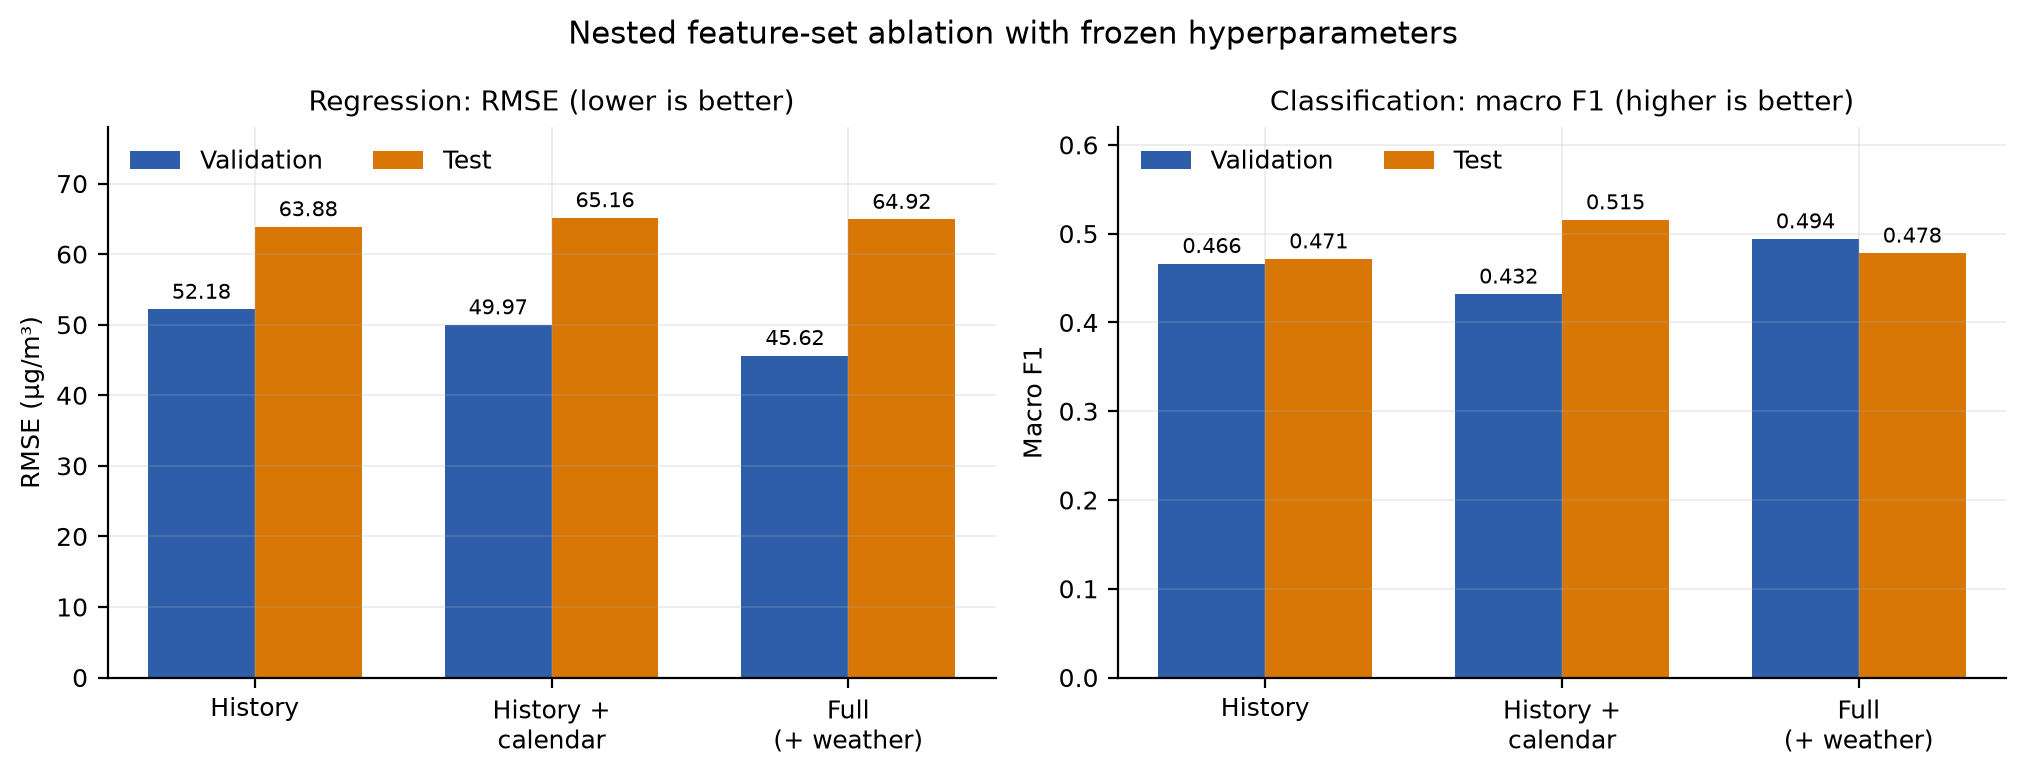
\includegraphics[width=\linewidth]{fig_ablation.png}
  \caption{Ablation results. The full model is best on validation for both tasks,
  but the test pattern is mixed: calendar features help classification and hurt
  regression, and the full model is not consistently best on test.}
  \label{fig:d3-ablation}
\end{figure}

The full model is best on validation for both tasks, which is why it is the
delivered model. The test pattern is mixed. Adding calendar features improves
classification test macro-F1 from 0.4715 to 0.5155 but lowers regression test
RMSE from 63.88 to 65.16. The full model then improves validation but gives back
some test performance. The honest conclusion is that there is no consistent
held-out gain from adding weather and calendar features on this dataset. The
ablation is descriptive, not a second model-selection step; switching to the
history-plus-calendar classifier after seeing test would violate the
validation-only rule.

\subsection{Backtest: 1 November 2024}
\label{sec:backtest}

A single backtest makes the application's limitations concrete. The feature date
is 1 November 2024, which is in the test split. Today's PM$_{2.5}$ is 156.6
$\mu$g/m$^3$. The app's six-input forecast is 159.23 $\mu$g/m$^3$, with an 80\%
interval of 101.7--209.7. The full-feature pipeline, using the actual history and
weather for that date, forecasts 188.23. The observed next-day PM$_{2.5}$ is
278.86. Persistence is 156.6. The actual value is outside the app's interval.

\begin{figure}[H]
  \centering
  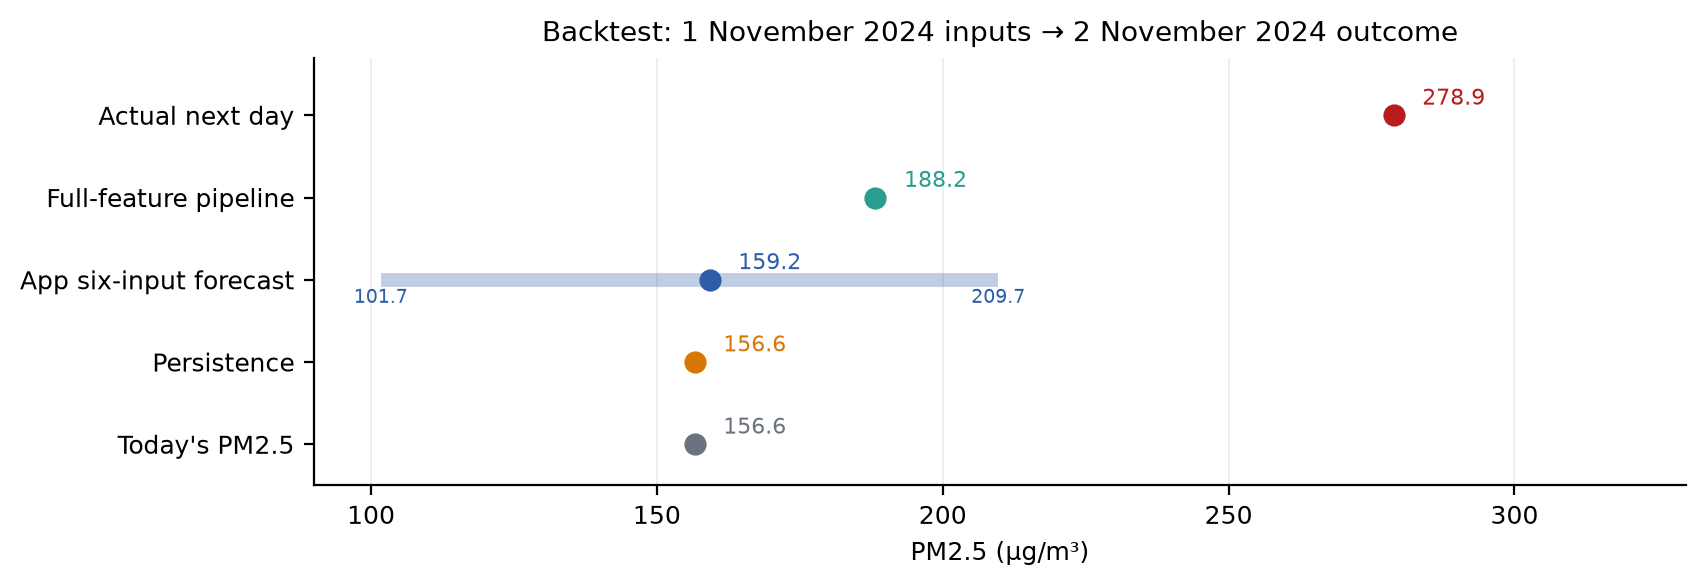
\includegraphics[width=0.96\linewidth]{fig_backtest.png}
  \caption{Backtest for 1 November 2024. The app forecast is close to
  persistence and far below the actual outcome; the full-feature model is
  closer but still under-predicts. This is the severe-tail failure that the bias
  analysis identified.}
  \label{fig:d3-backtest}
\end{figure}

\begin{table}[H]
\centering
\small
\begin{tabular}{@{}lr@{}}
\toprule
\textbf{Quantity} & \textbf{Value} \\
\midrule
Feature date & 1 November 2024 \\
Today's PM$_{2.5}$ & 156.6 $\mu$g/m$^3$ \\
App six-input forecast & 159.23 $\mu$g/m$^3$ \\
App 80\% interval & 101.7--209.7 $\mu$g/m$^3$ \\
Full-feature pipeline forecast & 188.23 $\mu$g/m$^3$ \\
Actual next-day PM$_{2.5}$ (2 November 2024) & 278.86 $\mu$g/m$^3$ \\
Persistence & 156.6 $\mu$g/m$^3$ \\
\bottomrule
\end{tabular}
\caption{Backtest for 1 November 2024. The app forecast and the full-feature
forecast both under-predict the severe day; the app's interval misses the
actual value.}
\label{tab:backtest}
\end{table}

The difference between 159.23 and 188.23 is informative. The app does not have
the actual previous days' PM$_{2.5}$ or the actual weather, so it assumes a
steady state and uses training medians for uncollected weather features. The
full-feature pipeline has the real inputs. Even with those inputs, it
under-predicts a severe day by about 91 $\mu$g/m$^3$. The app's lower forecast is
not evidence that the simpler interface is better; it is a consequence of
different information. The interval is wide, but not wide enough for this
outlier. With 77\% test coverage, some misses are expected; the important point
is that the miss is on a high-severity day, where the cost of under-prediction is
largest.

\subsection{What the app can and cannot claim}
\label{sec:claims}

Table~\ref{tab:claims} separates the defensible claims from the indefensible
ones. The app is a demonstration of an end-to-end explainable pipeline. It is not
an operational air-quality warning system.

\begin{table}[htbp]
\centering
\small
\begin{tabular}{@{}L{7.2cm}L{7.2cm}@{}}
\toprule
\textbf{The app can support} & \textbf{The app cannot support} \\
\midrule
A next-day PM$_{2.5}$ and AQI-category forecast from six inputs &
A claim that the forecast beats persistence on held-out data \\
A calibrated 80\% interval with reported validation and test coverage &
A guarantee that the interval contains the outcome \\
Local sensitivity and global permutation importance &
A causal claim about the effect of weather or policy \\
Seasonal context: monthly medians, stagnation, and the hourly profile &
A claim that winter afternoons are safe \\
A persistence comparison and a disagreement warning &
A claim that the classifier is reliable for rare hazardous classes \\
A reproducible artifact pipeline and 14 tests &
A live feed, a multi-day forecast, or a city-wide nowcast \\
Cautious, non-medical guidance &
Medical advice or a substitute for official advisories \\
\bottomrule
\end{tabular}
\caption{Defensible and indefensible claims for the Deliverable 3 application.}
\label{tab:claims}
\end{table}

\subsection{Limitations and ethics}
\label{sec:limitations-d3}

Table~\ref{tab:limitations-d3} consolidates the limitations from the model, the
data, and the application. The list is long because the project is deliberately
honest about what a single-station, six-input, one-day forecaster can do.

\begin{table}[htbp]
\centering
\footnotesize
\begin{tabular}{@{}L{3.8cm}L{5.7cm}L{5.5cm}@{}}
\toprule
\textbf{Limitation} & \textbf{Consequence} & \textbf{Mitigation or future work} \\
\midrule
One monitoring station & Results may not generalise to other neighbourhoods &
Add stations and a spatial validation design \\
Regression ties persistence; classifier loses & No evidence of an accuracy gain &
Report the baseline; treat the model as a demonstrator \\
Severe-tail under-prediction & The highest-risk days are the hardest &
Cost-sensitive training, quantile models, conformal intervals \\
Six inputs and many defaults & The forecast is illustrative, not live &
Ingest live weather and history; expose data provenance \\
Steady-state lags and rolling means & Rapid changes are under-represented &
Use the actual previous days' PM$_{2.5}$ \\
Classifier bias toward \emph{Unhealthy} & Category probabilities are overconfident &
Calibrate probabilities; use the implied category \\
80\% interval covers 77.0\% on test & Slight under-coverage &
Recalibrate on more data; add conformal prediction \\
Rare hazardous classes & Per-class metrics are noisy &
Collect more severe days; report support \\
Distribution shift & Validation-to-test reversals are possible &
Rolling-origin validation; monitor drift \\
No traffic data & Calendar features are proxies &
Integrate traffic and emissions data \\
Guidance is non-medical & Users may over-rely on the app &
Keep the disclaimer; link to official advisories \\
Single-station environmental justice & No demographic or neighbourhood fairness claim &
Add monitors and a population-aware evaluation \\
\bottomrule
\end{tabular}
\caption{Consolidated limitations and mitigations.}
\label{tab:limitations-d3}
\end{table}

\paragraph{Ethics.} The app processes no personal data and runs locally. If it
were deployed publicly, it would need authentication where appropriate, rate
limits, logging, a privacy review, and a clear separation between the
demonstration and official health advice. The guidance is intentionally
cautious: it tells users when to consider reducing exertion, not that a
particular activity is safe. The single-station limitation is also an equity
issue: a monitor at one location cannot represent the exposure of the whole
city, and the dataset contains no demographic attributes with which to test
fairness across groups.

\subsection{Reproducibility and repository guide}
\label{sec:repro-d3}

Table~\ref{tab:repro} lists the commands needed to rebuild the application and
the report from the committed source. All commands are run from the
\texttt{deliverable\_3} folder unless noted otherwise.

\begin{table}[H]
\centering
\footnotesize
\begin{tabular}{@{}L{3.2cm}L{7.4cm}L{4.0cm}@{}}
\toprule
\textbf{Step} & \textbf{Command} & \textbf{Expected output} \\
\midrule
Refit artifacts & \texttt{python -m src.train\_pipeline} &
Four joblib files and \texttt{metadata.json} \\
Run tests & \texttt{python -m unittest discover -s tests -t .} &
14 tests pass \\
Run ablation & \texttt{python -m src.ablation} &
\texttt{models/ablation.json} \\
Run app & \texttt{python -m streamlit run app/app.py} &
Local browser UI \\
Build figures & \texttt{python report/make\_figures.py} &
Report figures and \texttt{examples.json} \\
Build report & \texttt{tectonic report\_d3.tex} &
\texttt{report\_d3.pdf} \\
\bottomrule
\end{tabular}
\caption{Reproduction commands. The data files must be restored from the shared
Drive or regenerated from the data scripts before the refit. Append \texttt{-v}
to the test command for verbose output.}
\label{tab:repro}
\end{table}

The artifact policy is the same as in Deliverable 2: no fitted model binary and
no processed data file is committed. The \texttt{models/.gitignore} excludes the
joblib files, \texttt{metadata.json}, and \texttt{ablation.json}; the repository
root ignores the processed data. The refit is deterministic because the
hyperparameters and the random seed are fixed. The report figures are generated
from the persisted artifacts by \texttt{report/make\_figures.py}, so the report
and the app cannot silently diverge.

\paragraph{File map.} The D3 source is small enough to audit: \texttt{app/app.py}
is the interface; \texttt{src/inference.py} is the serving contract;
\texttt{src/train\_pipeline.py} refits the four pipelines and builds the
metadata; \texttt{src/ablation.py} runs the nested feature-set comparison;
\texttt{src/hourly.py} builds the hourly profile; \texttt{tests/test\_inference.py}
contains the 14 tests; \texttt{report/make\_figures.py} builds the report
figures; and \texttt{report/report\_d3.tex} is this report. The D1 and D2 reports
and code are unchanged.

\subsection{Conclusion and future work}
\label{sec:conclusion}

Deliverable 3 delivers a working, reproducible, explainable next-day air-quality
application for Lahore. The user enters six values; the app returns a PM$_{2.5}$
forecast, two category views, an 80\% interval, local and global explanations,
seasonal context, and a persistence comparison. The model is the frozen
Deliverable 2 model. It ties persistence on regression and loses to persistence
on classification macro-F1. The report does not hide that result, and the app
does not hide it either.

The most defensible contribution is the combination of a rigorous
validation-only modelling protocol, a calibrated uncertainty layer, an
explainable interface, a seasonal and hourly context, and a reproducibility
policy that regenerates every artifact from committed scripts. The project is
useful as a teaching and demonstration system, and as a foundation for a
stronger operational model.

Future work should proceed in the order that the evidence demands. First, ingest
live weather and PM$_{2.5}$ history so the inference layer does not rely on
steady-state assumptions. Second, add a second station and a rolling-origin
validation design to test whether the model generalises across place and time.
Third, improve the severe tail with cost-sensitive training, quantile or
conformal intervals, and a classifier that is calibrated rather than merely
arg-maxed. Fourth, replace the one-at-a-time sensitivity with a Shapley-value
decomposition if a more principled local explanation is needed. Finally, run a
small user study before making any public-health claim. Until then, the app
should remain a demonstration, and the official advisories should remain the
source of actionable guidance.
